%----------------------------------------------------------
% This is a substitute header file for Doxygen to use to generate the refman.tex file
%----------------------------------------------------------
%\batchmode
\documentclass[12pt,oneside]{book}
\usepackage{newclude}
\usepackage{a4wide}
\usepackage{makeidx}
\usepackage{graphicx}
\usepackage{multicol}
\usepackage{float}
\usepackage{listings}
\usepackage{color}
\usepackage{textcomp}
\usepackage{alltt}
\usepackage{times}
\usepackage{ifpdf}
\ifpdf
\usepackage[pdftex,
            pagebackref=true,
            colorlinks=true,
            linkcolor=blue,
            unicode
           ]{hyperref}
\else
\usepackage[ps2pdf,
            pagebackref=true,
            colorlinks=true,
            linkcolor=blue,
            unicode
           ]{hyperref}
\usepackage{pspicture}
\fi
\usepackage[utf8]{inputenc}
\usepackage{doxygen}
\lstset{language=C++,inputencoding=utf8,basicstyle=\footnotesize,breaklines=true,breakatwhitespace=true,tabsize=4,numbers=left }
\makeindex
\setcounter{tocdepth}{3}
\renewcommand{\footrulewidth}{0.4pt}

\textheight=9.0in
\textwidth=6.0in
\oddsidemargin=0.25in
\evensidemargin=0.0in
\topmargin=-0.5in


%----------------------------------------------------------
% Set the LaTex variables for the title page
%----------------------------------------------------------
\title{EMMPM Workbench}
\author{BlueQuartz Software}
\authoraddress{
  \url{http://www.bluequartz.net}\\
  Email: \email{mike.jackson@bluequartz.net}
}
\date{\today}

\hypersetup{pageanchor=false}

\begin{document}

\maketitle
    


%----------------------------------------------------------
% Set Table of Contents
%----------------------------------------------------------
%\clearemptydoublepage
\pagenumbering{roman}
\tableofcontents
\pagenumbering{arabic}
\hypersetup{pageanchor=true}

%----------------------------------------------------------
% This is the end of the header file
%----------------------------------------------------------

\chapter{Expectation Maximization/Maximization of Posterior Marginals}


\label{Expectation Maximization/Maximization of Posterior Marginals}
\hypertarget{Expectation Maximization/Maximization of Posterior Marginals}{}
\begin{figure}[htbp]
\begin{center}
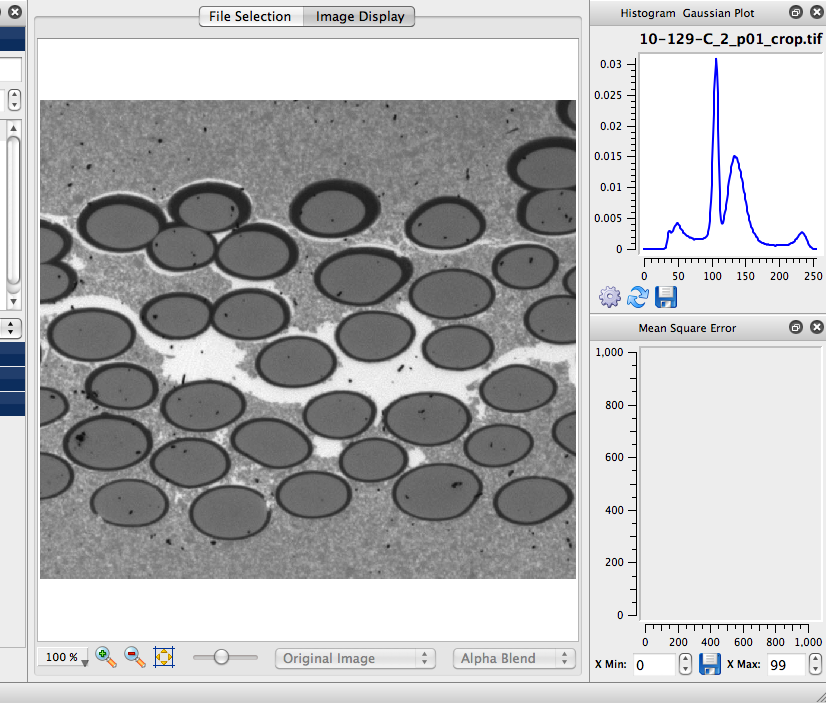
\includegraphics[width=6.0in]{images/UserInterface_3.png}
\caption{The EM/MPM Gui Image Display Area}
\label{UserInterface_3}
\end{center}
\end{figure}

One current research grade algorithm is the Expectation Maximization/ Maximization of Posterior Marginals (EM/MPM). A number of papers (\cite{1}, \cite{2}, \cite{3}) have been written on this technique and the explanations are better left to the developers. The basic premise is to use a mixture of Gaussian distributions to model the physical system. By knowing these various curves one can attempt to predict which pixel of an image should belong to which class designation. The basic EM/MPM algorithm is a nested loop structure with the outer loop being the EM loop and the inner loop being the MPM loop. Several input parameters control how the image is segmented and in the most basic version include the "Exchange Energy" and "Chemical Potential" terms. In advanced versions of the EM/MPM algorithm more parameters are available to the user. The EIM project selected this algorithm to be implemented in a more user friendly software package in combination with the enhancements made by other team members during the contracting period. This chapter will walk the new user through segmenting an example image starting with basic controls and moving to using the newer advanced options now available.

\section{Basic Input Parameters}

\begin{figure}[htbp]
\begin{center}
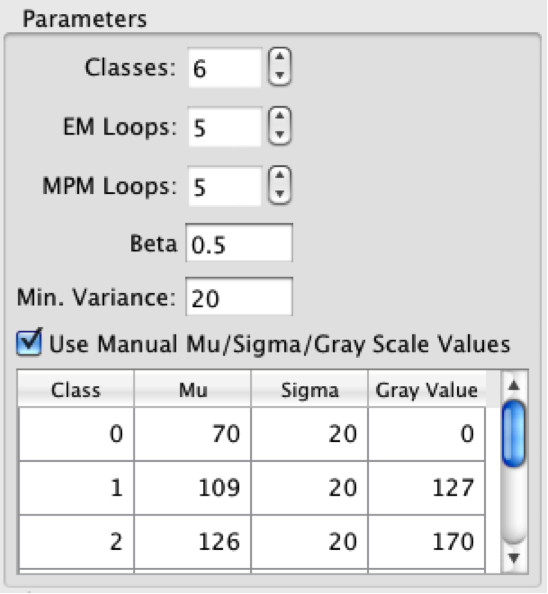
\includegraphics[width=3.25in]{images/Untitled3.png}
\caption{The EM/MPM Workbench Basic Inputs}
\label{image3}
\end{center}
\end{figure}

The basic inputs to the EM/MPM algorithm are the number of classes, the number of EM loops, the number of MPM loops, a Beta value and a Chemical Potential value. Taking each one of the parameters individually we have the following explanations: 
\begin{description}
\item[Classes:]This is the expected number of phases that can be segmented from the input image. In our example we use "2" because there is a darker epoxy based matrix surrounding a lighter Aluminum second phase. 
\item[Exchange Energy:]  The Exchange Energy, formerly called the Beta parameter, term controls how rough or smooth boundaries between each of the segmented phases will be. Another description is "... the spatial interaction parameter and is used to control how likely for two neighboring class labels to disagree."
\item[Histogram Loops:]  This controls the number of Expectation Maximization Loops that are performed. The EM Loops control how well the mixture of Gaussians model will fit the input image histogram. 
\item[Segmentation Loops:]  This controls the number of MPM loops that will be performed. The Segmentation loops control how well refined the final segmentation will be. 
\end{description}

Further "Per Class" parameters can also be set:
\begin{description}
\item[Chem. Pntl] This is the Chemical Potential, formerly called the "Chemical Potential" parameters.
\item[Color] This controls what color the specific class will show up as in the segmented image.
\item[Min. Std. Dev.:]  This is the minimum value of the standard deviation that will be allowed by the EM/MPM algorithm. The default is 4.5. Some segmentation runs may require this to be set higher or lower. If the histogram of the image shows peak areas that are narrow then a lower allowable standard deviation is needed for that class.
\end{description}


\section{Manual Initialization}
An additional checkbox {\bfseries Enable manual Initialization } allows the user to enter the initial Mean and Standard Deviation values for each class. As the user enters this information the histogram plot will automatically update with new estimated Gaussian curves. When these are filled out to the users satisfaction then the Segmentation can be started.
\begin{figure}[htbp]
\begin{center}
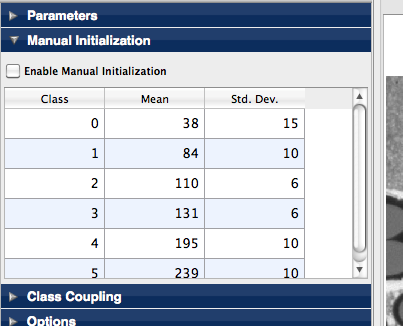
\includegraphics[width=3.5in]{images/Untitled5.png}
\caption{The EM/MPM Manual Initialization Table}
\label{Untitled5}
\end{center}
\end{figure}


\section{Class Coupling}
 We want to be able to ``couple'' a pair of classes together so that they segment differently. We allow the user to select the pair of classes by index (0 to N) and then assign a custom value for the Exchange Energy for those classes. We create a MxM matrix where M = number of classes + 1 and we fill it according to the following rules:
 
\begin{description}
\item[{\itshape 1}] Zero at [i,j] where i or j = Number of Classes
\item[{\itshape 2}] Global beta value from user for all classes in [i,j] where i or j != Number of classes
\item[{\itshape 3}] Custom beta value where i or j = either coupled class.
\end{description}
Using this option can help the segmentation where particles of different phases are close and either need to be prohibited from welding together or we actually want the particles to weld together.

\begin{figure}[htbp]
\begin{center}
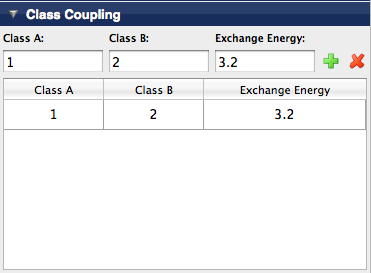
\includegraphics[width=3.5in]{images/Untitled14.png}
\caption{The Class Coupling Table}
\label{Untitled14}
\end{center}
\end{figure}

\section{Advanced Options}

\begin{figure}[htbp]
\begin{center}
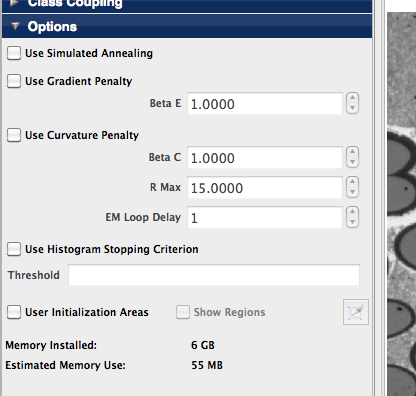
\includegraphics[width=3.5in]{images/Untitled4.png}
\caption{The EM/MPM Advanced Options}
\label{Untitled4}
\end{center}
\end{figure}
There are several additional options that the user can select that can effect the segmentation. 

\subsection{Simulated Annealing}
According to \cite{2} the following description of the "Simulated Annealing" is given. {\em The EM/MPM/SA algorithm was developed to form a preliminary segmentation with a low value of 'Beta', to classify textured regions, which is then progressively refined with larger and larger values of 'Beta' to sharpen the boundaries. In practice, a low value of 'Beta' is equivalent to choosing a high temperature, T , in equation  (\ref{eq:1}). A sufficient number of MPM cycles are run to provide a steady-state classification of pixels. Pixels that have a high probability of being classified as a single region tend to be stable, while those in which the probability of belonging to one of two or more different classes is uncertain tend to set up a dynamic equilibrium classification that changes as the MPM algorithm is executed. The pixels with high probability of classification are frozen in that class and the computation is not continued. Classification of the others continues at a lower temperature. The temperature is gradually lowered until pixel accuracy of classification of the boundaries is achieved.}

\begin{equation}
\label{eq:1}
Pr_i (ensemble image) = \frac{exp(-E_i/kT)}{\sum_{i}exp(-E_j/kT)}
\end{equation}

\subsection{Gradient Penalty}
This option attempts to apply a penalty function for large gray value gradients that occur at edges. More information about this penalty function can be found in \cite{4}.
\begin{description}
\item[Beta E:]  is a weight to control how much the edge cost information will be dominant in the classification process. Setting this value to Zero will have the same effect as disabling the option.
\end{description}

\subsection{Curvature Penalty}
This option applies a Curvature Penalty function in an attempt to smooth out boundaries between classes. The paper presented in \cite{4} is the best place for an in depth explanation of the implementation of the curvature penalty function.
\begin{description}
	\item[Beta C:]  A user-specified weight to control how much the curvature term dominates the classification process. Performing a morphological filtering using more than one structuring element incorporates the curvature penalty. Rather than using a single circular element, eight circular structuring elements with different radii are used. Setting this value to Zero will have the same effect as disabling the option. 
	\item[R Max:]  The maximum radius in pixels is specified by this parameter. 15 pixels seems to be a good starting point but note the larger this value is the slower the algorithm will run so the user should take into consideration any time constraints needed when running the program. 
	\item[EM Loop Delay:] This parameter is the number of EM loops to delay before applying this penalty function.
\end{description}

\subsection{Use Histogram Stopping Criterion}
For advanced users an option is available to stop the segmentation after a specific value for the Mean Square Error for the Sum of the MSE of the Mean and Standard Deviations is met (\ref{eq:2}).

\begin{equation}
\label{eq:2}
stopping = \sum_{j=0}^n(\mu_i - \mu_{(i-1)})^2 + \sum_{j=0}^n(\sigma_i^{2} - \sigma_{(i-1)}^{2})^2
\end{equation}

Most segmentations seem to hit a steady state with a "stopping value" < 1 after a number of "Histogram" (EM) Loops. It is up to the user to experiment to find this value. If the MSE value falls below the user supplied value then the segmentation will stop regardless of the number of "Histogram Loops" (EM Loops) have been executed. If the MSE value never falls below the user supplied value then the segmentation will stop after the set number of Histogram Loops have been executed.

\begin{figure}[htbp]
\begin{center}
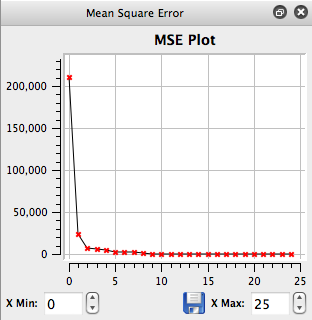
\includegraphics[width=3.3in]{images/Untitled13.png}
\caption{MSE Plot after a segmentation run of 25 EM Loops}
\label{Untitled13}
\end{center}
\end{figure}

\subsection{User Initialization Areas}
This option allows the user to designate areas of the image as having the approximate same mean and standard deviation of the final segmentation. This can be useful due to the algorithm used to pick the initial mean and standard deviation values. In some cases the model computed by the EM/MPM will not converge accurately to the image histogram.
 
\begin{figure}[htbp]
\begin{center}
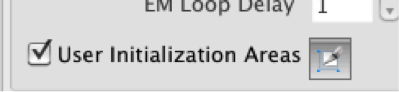
\includegraphics[width=5.0in]{images/Untitled8.png}
\caption{Enabling User Initialization Areas}
\label{image8}
\end{center}
\end{figure}

By designating similar areas for each phase the initial estimates for the mean and standard deviation become much more accurate. This should allow for a more accurate segmentation and also allow the user to need less EM loops, which will reduce the time needed to run the EM/MPM algorithm. To enable this option one needs to check the "User Initialization Areas" check box.
 

\begin{figure}[htbp]
\begin{center}
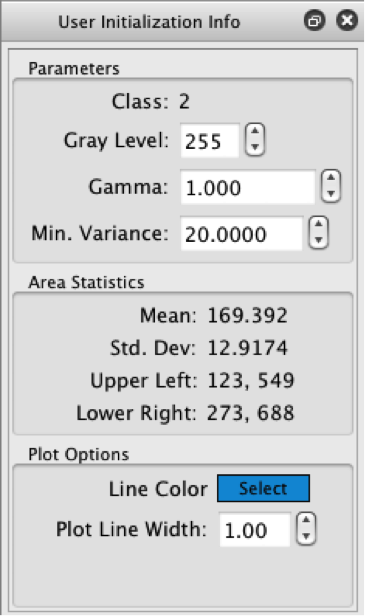
\includegraphics[width=3.00in]{images/Untitled9.png}
\caption{User Initialization Areas Widget}
\label{image9}
\end{center}
\end{figure}

To designate areas click on the "User Initialization Area Lasso Tool" and then draw out an area in the image by click dragging the outline of the area you want. If you do not get it exactly correct you can always resize and move the area after this operation. When you release the mouse button a dialog box will appear where you can set the initial values for that particular class. Because output images are saved as a <b>gray scale</b> image the setting of the Gray Level value is important at this point. While the defaults will attempt to spread out the values of the gray levels for each class sometimes this will create an image that is difficult for the human vision to discern differences between the various classes. The user should always take care to check this value for each class that they designate. Zero (0) means pure black and 255 means pure white. For a 2-class system the typical values that are used are 0 and 255. Setting the gray level to other values also has other implications that are discussed later on. By clicking/moving/resizing an individual area the details of that area will be displayed in the "User Initialization Info" palette. If the palette is not shown the user can use the Window menu to make it visible. 
Once the user has designated areas that represent each class the segmentation can then be run again to see if this has produced results that better match the intended segmentation. In this case the segmentation produces results where parts of the matrix are segmented as the light phase as shown in figure 1.12 where the left side of the image is the resulting segmentation of the right side of the image.
 

\begin{figure}[htbp]
\begin{center}
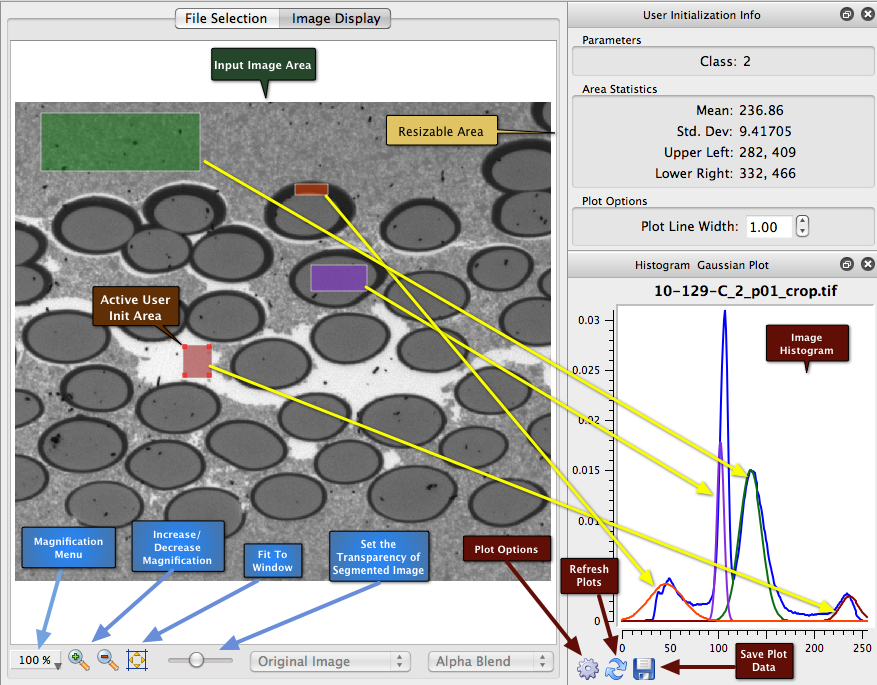
\includegraphics[width=6.25in]{images/Untitled10.png}
\caption{Detailed Callout of the User Interface}
\label{image10}
\end{center}
\end{figure}

Allowing the EM/MPM algorithm to use more classes to perform the segmentation then joining the classes into a single gray scale value when the final image is written can sometimes alleviate this type of segmentation error. This can be exactly achieved through adding an additional user initialization area but setting the output gray scale value to the same value (Zero in our example) as the matrix. Running the segmentation with all other values the same results in a segmentation that can be considered more accurate to the original input image.
 
\begin{figure}[htbp]
\begin{center}
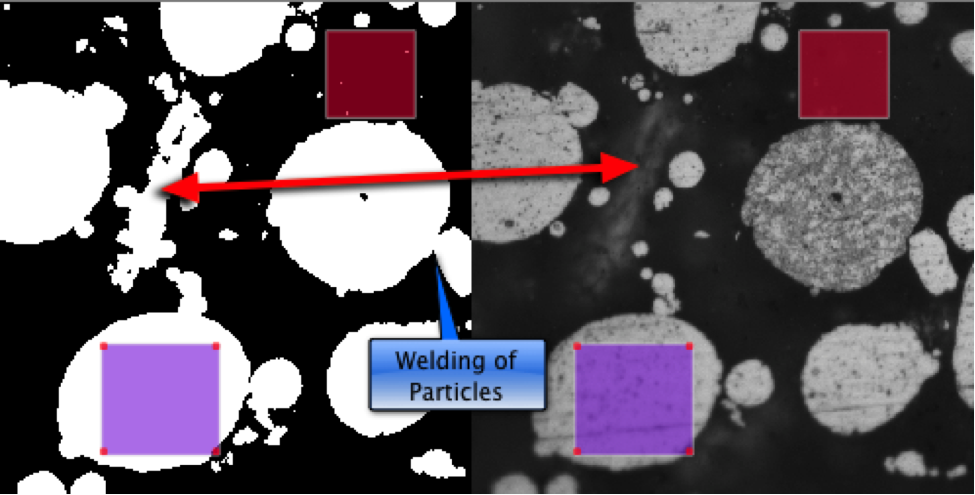
\includegraphics[width=6.25in]{images/Untitled11.png}
\caption{Initial Segmentation with 2 Classes allows parts of the matrix to be segmented as class 1}
\label{image11}
\end{center}
\end{figure}

Also note in the image that areas where the particles come close to each other but still have some matrix (class 0) between them get "welded" together in the first segmentation. In the second segmentation with the addition of another class the welding or joining of the particles does not happen. The last change from the first segmentation was the adjustment of the "Exchange Energy" value from 0.5 to 3.0. This allows some of the smaller holes to fill back in with the proper phase. 
 

\begin{figure}[htbp]
\begin{center}
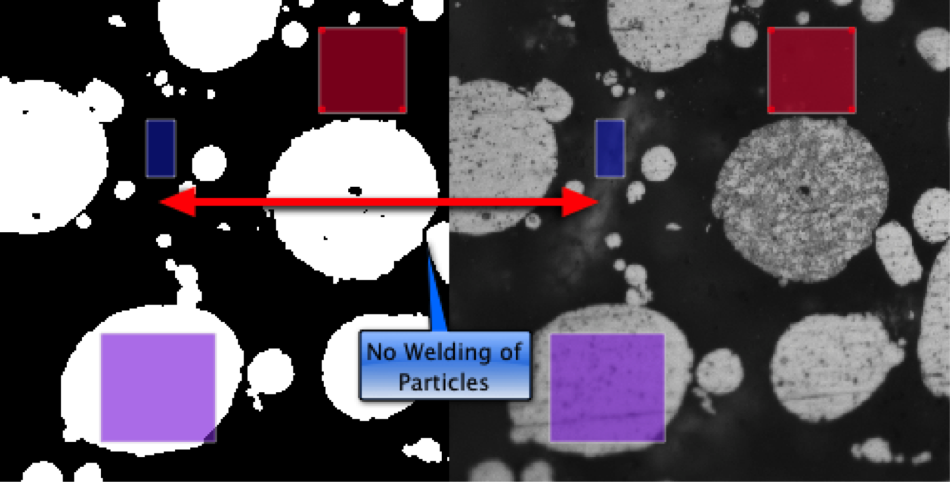
\includegraphics[width=6.25in]{images/Untitled12.png}
\caption{New segmentation with 3 classes results in more accurate results}
\label{image12}
\end{center}
\end{figure}

The ability to directly edit values in the "Parameters" area such as the Display Color and Chemical Potential value allows the user some flexibility on how the segmented image is saved. The Chemical Potential value has the effect that if a larger value is used for one class versus another then the EM/MPM will tend to assign the pixel to the class that has the larger Chemical Potential value instead of each class having equal probability as in the standard EM/MPM algorithm. Editing the color value can have interesting consequences in that the user can effectively segment with more than the final number of classes and have those classes automatically combined when the image is written by simply assigning the same color value for the classes that the user want to all contribute to the same final class in segmentation. For instance if the user wants a final binary segmentation with gray levels of zero and 255 but designates 4 total classes to use, 2 for the matrix and 2 for the phase, the user can set the two matrix classes to have a gray scale of 0 and the 2 phase classes to have a gray scale of 255. Even though the algorithm is using 4 classes the final image written to disk will only have 2 unique colors: 0 and 255. The final image is saved as an indexed image where the "image data" are the actual class values and a color lookup table is then supplied in the TIFF file. Advanced users can open this image in Photoshop or another image editor and replace the color table with their own specific color table.


%-----------------------------------------------------------
%
%-----------------------------------------------------------
\chapter{Running the Segmentation}

\section{Loading the Example Image}

\begin{figure}[htbp]
\begin{center}
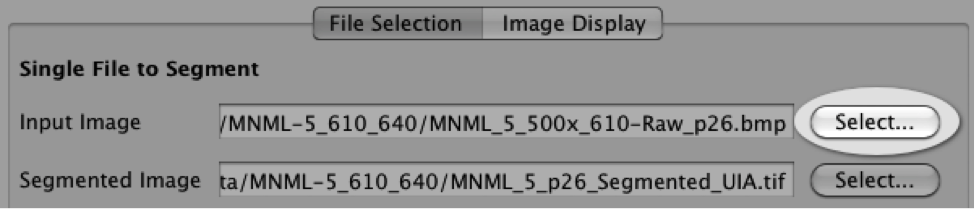
\includegraphics[width=4.0in]{images/Untitled1.png}
\caption{The EM/MPM Gui File Selection}
\label{image1}
\end{center}
\end{figure}

Click the "Select" button (See figure (\ref{image1}).) to display the "Open Input Image" file dialog box. After selecting the example image "MNML\_5\_500x\_610-Raw\_p26.bmp" from the examples directory click the "Open" button from the dialog and the image will be loaded into the EM/MPM Workbench. Click on the "Image Display" tab to view the input image (Figure 3.2). Within the "Image Display" tab there are two major sections that include the display of the selected input image and the display of the histogram of the input image. If the default values for the X and Y axis of the histogram are not appropriate to view the detail of the histogram the user can adjust these values using the text input fields found above the histogram plot. 

Now that we have selected our initial input values we can go ahead and run the segmentation. By clicking on the "Segment" button located below the inputs the image segmentation will start. 

During the segmentation the mixture of Gaussians will be updated on the same plot as the histogram as well as the evolving segmentation. The final segmentation is displayed in the Image Display Area. The red colored plot lines are the individual Gaussian distributions that the EM/MPM generated while the black line is the combined Gaussian distributions. In this case both the combined Gaussian and the individual Gaussian distributions are very close to the same values and so end up laying on top of each other. The separation is more evident as more classes are used to segment the image. 
 
 
\begin{figure}[htbp]
\begin{center}
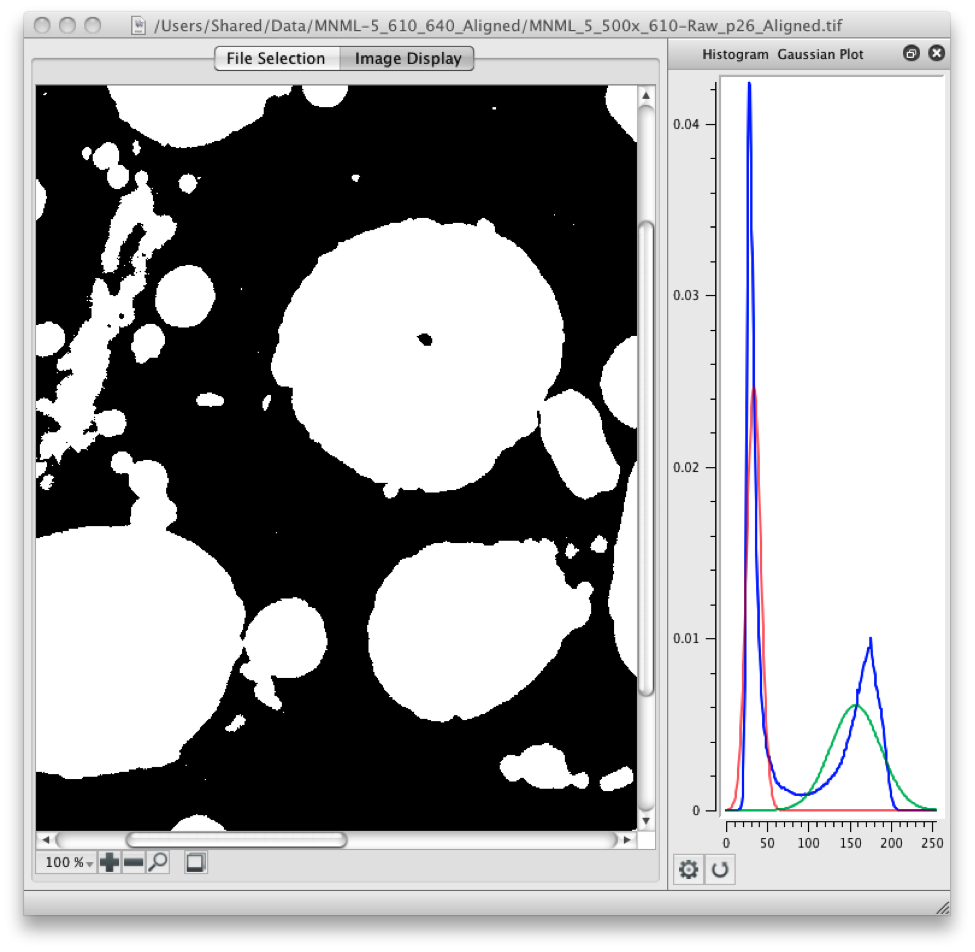
\includegraphics[width=6.0in]{images/Untitled6.png}
\caption{The EM/MPM Gui Output after Segmentation}
\label{image6}
\end{center}
\end{figure}

\chapter{Processing Multiple Images}
EMMPM Workbench allows the user to segment multiple images in one run. These images can be from a 3D stack of images possibly or from a 2D mosaic or just a bunch of images that are generally similar. The basic process is to first select an input directory that contains all the images. The use the filename filter to make sure only the images you want to have segmented are in the list. If you want to segment the images in a specific order the user can drag-n-drop files within the list to set a new order. The user should also select an output directory and optionally give the output files either a unique prefix and/or suffix. Some new options for processing multiple images is to use the final values for the Mean and Standard Deviation from the current image as the Initialization inputs into the next image. This gives the advantage of starting the next image with a mixture of Gaussians that is closer to the final mean and standard deviation values. This could potentially allow the user to use less EM loops to attain the same segmentation. Another option available is to output the mixture of Gaussian data along with the histogram to a CSV formatted file for each image. Some simple statistics are also output to a text file for each image that is segmented.
\begin{figure}[htbp]
\begin{center}
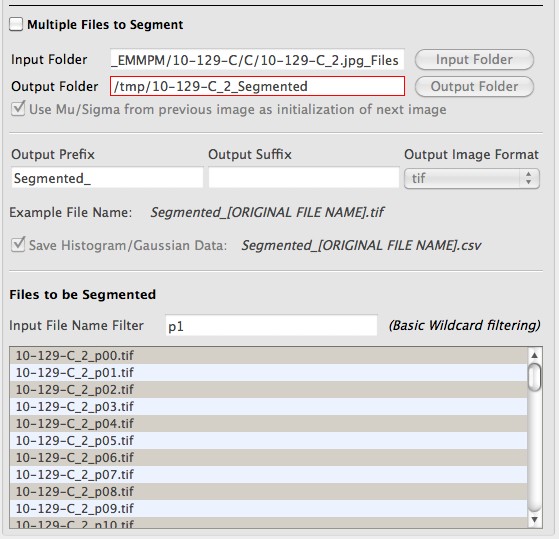
\includegraphics[width=6.4in]{images/Untitled15.png}
\caption{Processing Multiple Files}
\label{Untitled15}
\end{center}
\end{figure}

\chapter{Miscellanious Notes}

\section{Number of Classes}
Use more classes if you need more Gaussians to fit odd shaped peaks. In this sample, there are 2 peaks in the histogram and the method successfully fits two Gaussian peaks within it that gives a good segmentation.

\section{Histogram (EM) Loops}
Quality of optimization of the Gaussian fit to the histogram. Too few gives bad fit to histogram.

\section{Segmentation (MPM) Loops}
Controls the degree of convergence of the segmentation. Too few gives a speckled image.

\section{Exchange Energy (Beta)}
The Exchange Energy is the pairwise energy associated with a class mismatch
between two pixels and is always positive. Setting the Exchange Energy sets
this value for {\bfseries any} mismatch between two pixels. The Class Coupling allows
you to tailor this value for an interface between two specific classes. The
relative values of the Exchange Energies for the interfaces in an image
produces all of the capillarity effects that you would see with surface
tension.

\section{Chemical Potential (Gamma)}
The Chemical Potential is a thermodynamic variable that represents the free
energy change when a unit amount of an element is added to a mixture. In the
context of EM/MPM, the chemical potential is on a "per phase" basis, so
increasing the Chemical Potential increases the amount of that "phase." More
correctly, it increases the amount of the class for which the Chemical
Potential is set. Decreasing the Chemical Potential decreases that amount.
Note that, on the EM/MPM interface, the negative of the Chemical Potential
is given, so the numerical trend for -Chemical Potential is the opposite and
increasing this value can be viewed as penalizing the classification of
pixels into that class.

\subsection{Specific Strategies}

To increase an already segmented class by several pixels in the boundary
region, decrease the value of (-Chemical Potential) by a small amount.

To make small regions go away, increase the value of (-Chemical Potential)
and increase the value of the Exchange Energy between those regions and the
surrounding class.

To divide two different particles that are both embedded in a matrix,
increase the Exchange Energy between each of the particle classes and the
matrix, and decrease the Exchange Energy between the two particles. It may
be necessary to decrease the (-Chemical Potential) of the matrix phase.

To fuse two different particles that are embedded in a matrix, do the
opposite.

\section{Simulated Annealing}
Simulated annealing raises the Beta value as the segmentation goes on. On samples with really fine channels, it tends to weld things together because of capillarity (Beta is the pairwise interaction between pixels. Really large values of Beta simulate real large interfacial energies. Regions in contact tend to grow together to remove interfacial energy). Not using simulated annealing can lead to speckled images. Using it can lead to particle welding.
\section{Edge Gradient Penalty}
The gradient penalty detects systematic drops in intensity and allows you to split the particles apart, even though the intensity in the channel doesn't ever drop to what you would put as a threshold. Not using a gradient penalty can lead to intensity dips being smoothed out. Using too high a gradient penalty can cause individual pixels to be segmented because of Poisson noise that changes their intensity vis a vis neighboring pixels.
\section{Beta E}
Segmentation is very sensitive to Beta E values. On some samples, you have a lot of Poisson noise, and it's not useful to raise Beta E above maybe 2 or 3. If you do, you just get sand, because it splits the high brightness pixels from their neighbors. Too low a Beta E can lead to jaggy boundaries.
\section{Curvature Penalty}
There are two ways of smoothing a curve: raising Beta E and applying a curvature penalty. Raising Beta E makes particles consolidate, Curvature penalties do not.
\section{Beta C}
You may be able to get smoother boundaries by increasing this value, but morphological filtering does not have prior knowledge in it. If you get unrealistic segmentations with Beta C, they will show more about the actual structuring element used in the morphological filter than the material or prior knowledge. Too high a value of Beta C can lead to unrealistically shaped particles. Too low can lead to jaggy edges that you're tempted to smooth out with Beta E increases, which causes particles to weld.
\section{R Max}
R Max is (roughly) the maximum number of pixels you can erode back from the boundary. You have to use a larger value of Beta C if you use a smaller value of R Max. Larger R Max values lead to longer segmentation times. Too low a value can lead to jaggy interfaces. Too high can lead to excessive wait times for segmentations.

\newpage
\begin{thebibliography}{4}

\bibitem{1}
Mary L. Comer
\newblock The EM/MPM Algorithm for Segmentation of Textured Images: Analysis and Further Experimental Results
\newblock {\em IEEE TRANSACTIONS ON IMAGE PROCESSING}, VOL. 9, NO. 10, OCTOBER 2000.


\bibitem{2} 
J P Simmons, P Chuang, M Comer, J E Spowart, M D Uchic and M De Graef
\newblock Application and further development of advanced image processing algorithms for automated analysis of serial section image data, 
\newblock {\em Modelling Simul. Mater. Sci. Eng.} 17 (2009). 


\bibitem{3} 
David Doria, 
\newblock Expectation Maximization of Gaussian Mixture Models in VTK - Release 0.00, September 21, 2010
\newblock { \em Insight Journal} [http://hdl.handle.net/10380/3218] 


 \bibitem{4} 
J. Dumke and M. Comer, 
\newblock Automated segmentation of alloy microstructures in serial section images
\newblock { \em Proceedings of SPIE}, vol. 6498, p. 64980E, 2007

\end{thebibliography}
%---------------
% 
%---------------

\printindex
\end{document}
